

\tikzset{every picture/.style={line width=0.75pt}} %set default line width to 0.75pt        

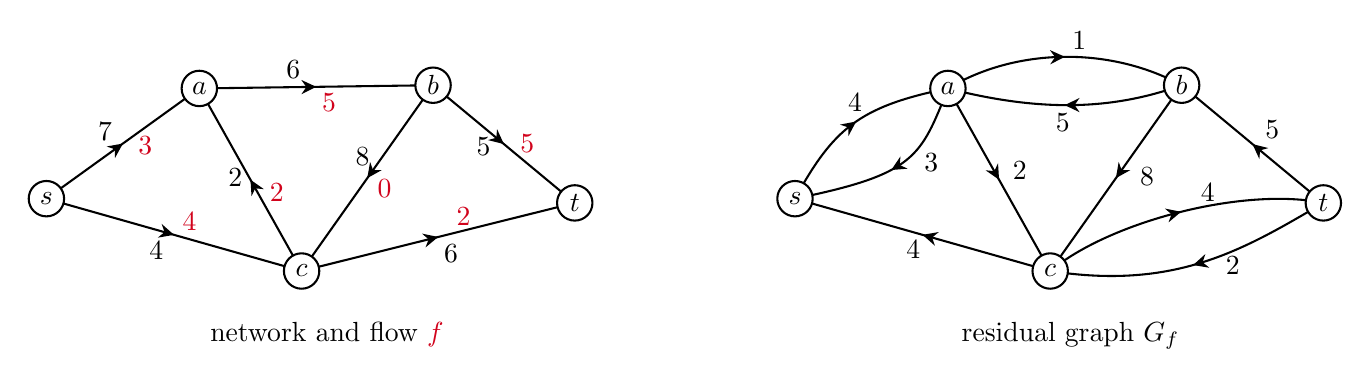
\begin{tikzpicture}[x=0.5pt,y=0.5pt,yscale=-1,xscale=1]
%uncomment if require: \path (0,249); %set diagram left start at 0, and has height of 249

%Curve Lines [id:da5613638706519646] 
\draw    (745.22,183) .. controls (788.5,147) and (885.5,122) .. (942.62,133.78) ;
\draw [shift={(839.83,140.2)}, rotate = 525.5699999999999] [fill={rgb, 255:red, 0; green, 0; blue, 0 }  ][line width=0.08]  [draw opacity=0] (10.72,-5.15) -- (0,0) -- (10.72,5.15) -- (7.12,0) -- cycle    ;
%Curve Lines [id:da2735285843771139] 
\draw    (560.79,130.72) .. controls (588.5,80) and (607.5,64) .. (671.31,51.06) ;
\draw [shift={(604.98,74.96)}, rotate = 503.55] [fill={rgb, 255:red, 0; green, 0; blue, 0 }  ][line width=0.08]  [draw opacity=0] (10.72,-5.15) -- (0,0) -- (10.72,5.15) -- (7.12,0) -- cycle    ;
%Curve Lines [id:da6525683976596537] 
\draw    (671.31,51.06) .. controls (651.5,101) and (647.5,113) .. (560.79,130.72) ;
\draw [shift={(630.35,110.01)}, rotate = 329.68] [fill={rgb, 255:red, 0; green, 0; blue, 0 }  ][line width=0.08]  [draw opacity=0] (10.72,-5.15) -- (0,0) -- (10.72,5.15) -- (7.12,0) -- cycle    ;
%Curve Lines [id:da9916324740026169] 
\draw    (671.31,51.06) .. controls (719.5,22) and (787.5,20) .. (840.22,48.73) ;
\draw [shift={(755.84,28.2)}, rotate = 538.53] [fill={rgb, 255:red, 0; green, 0; blue, 0 }  ][line width=0.08]  [draw opacity=0] (10.72,-5.15) -- (0,0) -- (10.72,5.15) -- (7.12,0) -- cycle    ;
%Curve Lines [id:da8306124055787136] 
\draw    (840.22,48.73) .. controls (789.5,67) and (737.5,68) .. (671.31,51.06) ;
\draw [shift={(755.74,63.12)}, rotate = 359.78] [fill={rgb, 255:red, 0; green, 0; blue, 0 }  ][line width=0.08]  [draw opacity=0] (10.72,-5.15) -- (0,0) -- (10.72,5.15) -- (7.12,0) -- cycle    ;
%Curve Lines [id:da21823822635678936] 
\draw    (942.62,133.78) .. controls (884.5,168) and (835.5,197) .. (745.22,183) ;
\draw [shift={(848.51,178.7)}, rotate = 343.65] [fill={rgb, 255:red, 0; green, 0; blue, 0 }  ][line width=0.08]  [draw opacity=0] (10.72,-5.15) -- (0,0) -- (10.72,5.15) -- (7.12,0) -- cycle    ;
%Straight Lines [id:da06700183790814418] 
\draw    (745.22,183) -- (840.22,48.73) ;
\draw [shift={(792.72,115.86)}, rotate = 305.28] [fill={rgb, 255:red, 0; green, 0; blue, 0 }  ][line width=0.08]  [draw opacity=0] (10.72,-5.15) -- (0,0) -- (10.72,5.15) -- (7.12,0) -- cycle    ;
%Straight Lines [id:da78660649581525] 
\draw    (671.31,51.06) -- (745.22,183) ;
\draw [shift={(708.27,117.03)}, rotate = 240.74] [fill={rgb, 255:red, 0; green, 0; blue, 0 }  ][line width=0.08]  [draw opacity=0] (10.72,-5.15) -- (0,0) -- (10.72,5.15) -- (7.12,0) -- cycle    ;
%Straight Lines [id:da8749205218684325] 
\draw    (745.22,183) -- (560.79,130.72) ;
\draw [shift={(653.01,156.86)}, rotate = 375.83000000000004] [fill={rgb, 255:red, 0; green, 0; blue, 0 }  ][line width=0.08]  [draw opacity=0] (10.72,-5.15) -- (0,0) -- (10.72,5.15) -- (7.12,0) -- cycle    ;
%Straight Lines [id:da4360222788208358] 
\draw    (840.22,48.73) -- (942.62,133.78) ;
\draw [shift={(891.42,91.26)}, rotate = 39.71] [fill={rgb, 255:red, 0; green, 0; blue, 0 }  ][line width=0.08]  [draw opacity=0] (10.72,-5.15) -- (0,0) -- (10.72,5.15) -- (7.12,0) -- cycle    ;
%Shape: Ellipse [id:dp22199319065994672] 
\draw  [fill={rgb, 255:red, 255; green, 255; blue, 255 }  ,fill opacity=1 ] (548,130.72) .. controls (548,123.66) and (553.73,117.93) .. (560.79,117.93) .. controls (567.86,117.93) and (573.58,123.66) .. (573.58,130.72) .. controls (573.58,137.78) and (567.86,143.51) .. (560.79,143.51) .. controls (553.73,143.51) and (548,137.78) .. (548,130.72) -- cycle ;
%Shape: Ellipse [id:dp734016786907147] 
\draw  [fill={rgb, 255:red, 255; green, 255; blue, 255 }  ,fill opacity=1 ] (658.52,51.06) .. controls (658.52,44) and (664.25,38.27) .. (671.31,38.27) .. controls (678.38,38.27) and (684.1,44) .. (684.1,51.06) .. controls (684.1,58.13) and (678.38,63.85) .. (671.31,63.85) .. controls (664.25,63.85) and (658.52,58.13) .. (658.52,51.06) -- cycle ;
%Shape: Ellipse [id:dp6263378369405302] 
\draw  [fill={rgb, 255:red, 255; green, 255; blue, 255 }  ,fill opacity=1 ] (827.43,48.73) .. controls (827.43,41.66) and (833.15,35.94) .. (840.22,35.94) .. controls (847.28,35.94) and (853.01,41.66) .. (853.01,48.73) .. controls (853.01,55.79) and (847.28,61.52) .. (840.22,61.52) .. controls (833.15,61.52) and (827.43,55.79) .. (827.43,48.73) -- cycle ;
%Shape: Ellipse [id:dp7990256965184968] 
\draw  [fill={rgb, 255:red, 255; green, 255; blue, 255 }  ,fill opacity=1 ] (732.43,183) .. controls (732.43,175.94) and (738.15,170.21) .. (745.22,170.21) .. controls (752.28,170.21) and (758.01,175.94) .. (758.01,183) .. controls (758.01,190.06) and (752.28,195.79) .. (745.22,195.79) .. controls (738.15,195.79) and (732.43,190.06) .. (732.43,183) -- cycle ;
%Shape: Ellipse [id:dp7073963568621764] 
\draw  [fill={rgb, 255:red, 255; green, 255; blue, 255 }  ,fill opacity=1 ] (929.83,133.78) .. controls (929.83,126.72) and (935.56,120.99) .. (942.62,120.99) .. controls (949.69,120.99) and (955.41,126.72) .. (955.41,133.78) .. controls (955.41,140.85) and (949.69,146.57) .. (942.62,146.57) .. controls (935.56,146.57) and (929.83,140.85) .. (929.83,133.78) -- cycle ;

%Straight Lines [id:da5195310081734267] 
\draw    (204.22,183) -- (299.22,48.73) ;
\draw [shift={(251.72,115.86)}, rotate = 305.28] [fill={rgb, 255:red, 0; green, 0; blue, 0 }  ][line width=0.08]  [draw opacity=0] (10.72,-5.15) -- (0,0) -- (10.72,5.15) -- (7.12,0) -- cycle    ;
%Straight Lines [id:da4538291997735936] 
\draw    (130.31,51.06) -- (204.22,183) ;
\draw [shift={(167.27,117.03)}, rotate = 60.74] [fill={rgb, 255:red, 0; green, 0; blue, 0 }  ][line width=0.08]  [draw opacity=0] (10.72,-5.15) -- (0,0) -- (10.72,5.15) -- (7.12,0) -- cycle    ;
%Straight Lines [id:da7538382565478482] 
\draw    (19.79,130.72) -- (204.22,183) ;
\draw [shift={(112.01,156.86)}, rotate = 195.83] [fill={rgb, 255:red, 0; green, 0; blue, 0 }  ][line width=0.08]  [draw opacity=0] (10.72,-5.15) -- (0,0) -- (10.72,5.15) -- (7.12,0) -- cycle    ;
%Straight Lines [id:da6748069532380702] 
\draw    (401.62,133.78) -- (204.22,183) ;
\draw [shift={(302.92,158.39)}, rotate = 166] [fill={rgb, 255:red, 0; green, 0; blue, 0 }  ][line width=0.08]  [draw opacity=0] (10.72,-5.15) -- (0,0) -- (10.72,5.15) -- (7.12,0) -- cycle    ;
%Straight Lines [id:da3976427132067899] 
\draw    (19.79,130.72) -- (130.31,51.06) ;
\draw [shift={(75.05,90.89)}, rotate = 504.22] [fill={rgb, 255:red, 0; green, 0; blue, 0 }  ][line width=0.08]  [draw opacity=0] (10.72,-5.15) -- (0,0) -- (10.72,5.15) -- (7.12,0) -- cycle    ;
%Straight Lines [id:da5989756628707282] 
\draw    (299.22,48.73) -- (401.62,133.78) ;
\draw [shift={(350.42,91.26)}, rotate = 219.71] [fill={rgb, 255:red, 0; green, 0; blue, 0 }  ][line width=0.08]  [draw opacity=0] (10.72,-5.15) -- (0,0) -- (10.72,5.15) -- (7.12,0) -- cycle    ;
%Straight Lines [id:da8582315780180115] 
\draw    (130.31,51.06) -- (299.22,48.73) ;
\draw [shift={(214.76,49.89)}, rotate = 539.21] [fill={rgb, 255:red, 0; green, 0; blue, 0 }  ][line width=0.08]  [draw opacity=0] (10.72,-5.15) -- (0,0) -- (10.72,5.15) -- (7.12,0) -- cycle    ;
%Shape: Ellipse [id:dp48011285603633225] 
\draw  [fill={rgb, 255:red, 255; green, 255; blue, 255 }  ,fill opacity=1 ] (7,130.72) .. controls (7,123.66) and (12.73,117.93) .. (19.79,117.93) .. controls (26.86,117.93) and (32.58,123.66) .. (32.58,130.72) .. controls (32.58,137.78) and (26.86,143.51) .. (19.79,143.51) .. controls (12.73,143.51) and (7,137.78) .. (7,130.72) -- cycle ;
%Shape: Ellipse [id:dp34527564053657145] 
\draw  [fill={rgb, 255:red, 255; green, 255; blue, 255 }  ,fill opacity=1 ] (117.52,51.06) .. controls (117.52,44) and (123.25,38.27) .. (130.31,38.27) .. controls (137.38,38.27) and (143.1,44) .. (143.1,51.06) .. controls (143.1,58.13) and (137.38,63.85) .. (130.31,63.85) .. controls (123.25,63.85) and (117.52,58.13) .. (117.52,51.06) -- cycle ;
%Shape: Ellipse [id:dp6239749822676505] 
\draw  [fill={rgb, 255:red, 255; green, 255; blue, 255 }  ,fill opacity=1 ] (286.43,48.73) .. controls (286.43,41.66) and (292.15,35.94) .. (299.22,35.94) .. controls (306.28,35.94) and (312.01,41.66) .. (312.01,48.73) .. controls (312.01,55.79) and (306.28,61.52) .. (299.22,61.52) .. controls (292.15,61.52) and (286.43,55.79) .. (286.43,48.73) -- cycle ;
%Shape: Ellipse [id:dp4869792682336288] 
\draw  [fill={rgb, 255:red, 255; green, 255; blue, 255 }  ,fill opacity=1 ] (191.43,183) .. controls (191.43,175.94) and (197.15,170.21) .. (204.22,170.21) .. controls (211.28,170.21) and (217.01,175.94) .. (217.01,183) .. controls (217.01,190.06) and (211.28,195.79) .. (204.22,195.79) .. controls (197.15,195.79) and (191.43,190.06) .. (191.43,183) -- cycle ;
%Shape: Ellipse [id:dp8101897126294262] 
\draw  [fill={rgb, 255:red, 255; green, 255; blue, 255 }  ,fill opacity=1 ] (388.83,133.78) .. controls (388.83,126.72) and (394.56,120.99) .. (401.62,120.99) .. controls (408.69,120.99) and (414.41,126.72) .. (414.41,133.78) .. controls (414.41,140.85) and (408.69,146.57) .. (401.62,146.57) .. controls (394.56,146.57) and (388.83,140.85) .. (388.83,133.78) -- cycle ;


% Text Node
\draw (136,217.5) node [anchor=north west][inner sep=0.75pt]   [align=left] {network and flow $\displaystyle \textcolor[rgb]{0.82,0.01,0.11}{f}$};
% Text Node
\draw (679,217.5) node [anchor=north west][inner sep=0.75pt]   [align=left] {residual graph $\displaystyle G_{f}$};
% Text Node
\draw (19.79,130.72) node   [align=left] {$\displaystyle s$};
% Text Node
\draw (130.31,51.06) node   [align=left] {$\displaystyle a$};
% Text Node
\draw (299.22,48.73) node   [align=left] {$\displaystyle b$};
% Text Node
\draw (204.22,183) node   [align=left] {$\displaystyle c$};
% Text Node
\draw (401.62,133.78) node   [align=left] {$\displaystyle t$};
% Text Node
\draw (92,159.89) node [anchor=north west][inner sep=0.75pt]   [align=left] {$\displaystyle 4$};
% Text Node
\draw (241,91.89) node [anchor=north west][inner sep=0.75pt]   [align=left] {$\displaystyle 8$};
% Text Node
\draw (149,106.89) node [anchor=north west][inner sep=0.75pt]   [align=left] {$\displaystyle 2$};
% Text Node
\draw (55,73.89) node [anchor=north west][inner sep=0.75pt]   [align=left] {$\displaystyle 7$};
% Text Node
\draw (304.92,161.39) node [anchor=north west][inner sep=0.75pt]   [align=left] {$\displaystyle 6$};
% Text Node
\draw (328.42,84.26) node [anchor=north west][inner sep=0.75pt]   [align=left] {$\displaystyle 5$};
% Text Node
\draw (191,28.89) node [anchor=north west][inner sep=0.75pt]   [align=left] {$\displaystyle 6$};
% Text Node
\draw (116,138.89) node [anchor=north west][inner sep=0.75pt]   [align=left] {$\displaystyle \textcolor[rgb]{0.82,0.01,0.11}{4}$};
% Text Node
\draw (179,117.89) node [anchor=north west][inner sep=0.75pt]   [align=left] {$\displaystyle \textcolor[rgb]{0.82,0.01,0.11}{2}$};
% Text Node
\draw (314,134.89) node [anchor=north west][inner sep=0.75pt]   [align=left] {$\displaystyle \textcolor[rgb]{0.82,0.01,0.11}{2}$};
% Text Node
\draw (84,83.89) node [anchor=north west][inner sep=0.75pt]   [align=left] {$\displaystyle \textcolor[rgb]{0.82,0.01,0.11}{3}$};
% Text Node
\draw (216.76,52.89) node [anchor=north west][inner sep=0.75pt]   [align=left] {$\displaystyle \textcolor[rgb]{0.82,0.01,0.11}{5}$};
% Text Node
\draw (257,114.89) node [anchor=north west][inner sep=0.75pt]   [align=left] {$\displaystyle \textcolor[rgb]{0.82,0.01,0.11}{0}$};
% Text Node
\draw (360,81.89) node [anchor=north west][inner sep=0.75pt]   [align=left] {$\displaystyle \textcolor[rgb]{0.82,0.01,0.11}{5}$};
% Text Node
\draw (560.79,130.72) node   [align=left] {$\displaystyle s$};
% Text Node
\draw (671.31,51.06) node   [align=left] {$\displaystyle a$};
% Text Node
\draw (840.22,48.73) node   [align=left] {$\displaystyle b$};
% Text Node
\draw (745.22,183) node   [align=left] {$\displaystyle c$};
% Text Node
\draw (942.62,133.78) node   [align=left] {$\displaystyle t$};
% Text Node
\draw (652,95.89) node [anchor=north west][inner sep=0.75pt]   [align=left] {$\displaystyle 3$};
% Text Node
\draw (808,105.89) node [anchor=north west][inner sep=0.75pt]   [align=left] {$\displaystyle 8$};
% Text Node
\draw (716,101.89) node [anchor=north west][inner sep=0.75pt]   [align=left] {$\displaystyle 2$};
% Text Node
\draw (597,52.89) node [anchor=north west][inner sep=0.75pt]   [align=left] {$\displaystyle 4$};
% Text Node
\draw (851.92,117.39) node [anchor=north west][inner sep=0.75pt]   [align=left] {$\displaystyle 4$};
% Text Node
\draw (898.42,72.26) node [anchor=north west][inner sep=0.75pt]   [align=left] {$\displaystyle 5$};
% Text Node
\draw (759,7.89) node [anchor=north west][inner sep=0.75pt]   [align=left] {$\displaystyle 1$};
% Text Node
\draw (639,158.89) node [anchor=north west][inner sep=0.75pt]   [align=left] {$\displaystyle 4$};
% Text Node
\draw (747,66.89) node [anchor=north west][inner sep=0.75pt]   [align=left] {$\displaystyle 5$};
% Text Node
\draw (869.92,170.39) node [anchor=north west][inner sep=0.75pt]   [align=left] {$\displaystyle 2$};


\end{tikzpicture}

